\begin{pastexam}[label={px:gw3-114-ds-03}]{關務三等資訊處理 114 年 第三題}
（申論；25 分）

假設現有五個字母 A, B, C, D, E 的頻率分別為 0.19, 0.09, 0.21, 0.12, 0.39，請依步驟建構霍夫曼樹（Huffman
Tree）。（25 分）
\end{pastexam}

\begin{pastsoln}
\textbf{方法}（資結書第~19.3~節）：每個字母是一個節點，權重是頻率。 每一步取出權重最小的兩個，合併成
一個新節點（權重相加），較小的當左子、較大的當右子，放回去；做 $5 - 1 = 4$ 次就剩一棵樹。 最後左邊記
$0$、右邊記 $1$ 得到編碼。 平手時本解答先取原本就在的節點（新合併出來的排在同權重的後面）；別的取法
樹形可能不同，但每個字母的編碼長度、平均長度都一樣是最佳的。

\textbf{步驟}（每步後列出目前的節點，由小到大）：
\begin{center}
\begin{tabular}{clll}
\toprule
步 & 取出 & 合併成 & 剩下的節點 \\
\midrule
0 & & & B 0.09, D 0.12, A 0.19, C 0.21, E 0.39 \\
1 & B 0.09, D 0.12 & (BD) 0.21 & A 0.19, C 0.21, (BD) 0.21, E 0.39 \\
2 & A 0.19, C 0.21 & (AC) 0.40 & (BD) 0.21, E 0.39, (AC) 0.40 \\
3 & (BD) 0.21, E 0.39 & (BDE) 0.60 & (AC) 0.40, (BDE) 0.60 \\
4 & (AC) 0.40, (BDE) 0.60 & 根 1.00 & 根 1.00 \\
\bottomrule
\end{tabular}
\end{center}
第 2 步 C 和 (BD) 都是 $0.21$，平手，依上面的約定先取 C。

\textbf{霍夫曼樹}（左邊的邊記 $0$、右邊記 $1$）：
\begin{center}
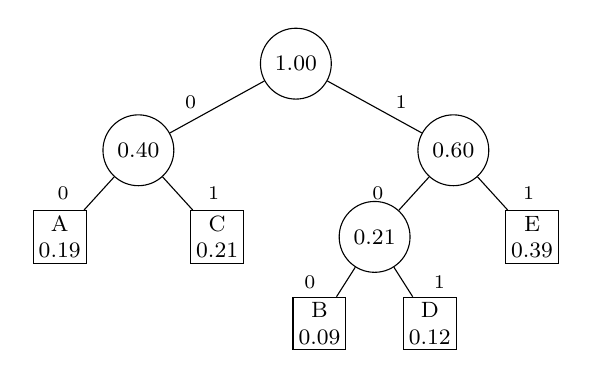
\begin{tikzpicture}[level distance=11mm,
  level 1/.style={sibling distance=40mm}, level 2/.style={sibling distance=20mm},
  level 3/.style={sibling distance=14mm},
  every node/.style={circle, draw, minimum size=9mm, inner sep=0pt, font=\footnotesize},
  lf/.style={rectangle, draw, minimum size=6mm, inner sep=2pt, align=center, font=\footnotesize},
  edge from parent/.style={draw},
  b/.style={draw=none, rectangle, font=\scriptsize, inner sep=1pt}]
\node {1.00}
  child {node {0.40}
    child {node[lf] {A\\0.19} edge from parent node[b, left] {0}}
    child {node[lf] {C\\0.21} edge from parent node[b, right] {1}}
    edge from parent node[b, left, pos=0.4] {0}}
  child {node {0.60}
    child {node {0.21}
      child {node[lf] {B\\0.09} edge from parent node[b, left] {0}}
      child {node[lf] {D\\0.12} edge from parent node[b, right] {1}}
      edge from parent node[b, left] {0}}
    child {node[lf] {E\\0.39} edge from parent node[b, right] {1}}
    edge from parent node[b, right, pos=0.4] {1}};
\end{tikzpicture}
\end{center}

\textbf{編碼與平均長度}：
\begin{center}
\begin{tabular}{cccc}
\toprule
字母 & 頻率 & 編碼 & 長度 \\
\midrule
A & 0.19 & 00 & 2 \\
B & 0.09 & 100 & 3 \\
C & 0.21 & 01 & 2 \\
D & 0.12 & 101 & 3 \\
E & 0.39 & 11 & 2 \\
\bottomrule
\end{tabular}
\end{center}
平均編碼長度 $= 0.19 \cdot 2 + 0.09 \cdot 3 + 0.21 \cdot 2 + 0.12 \cdot 3 + 0.39 \cdot 2 = 0.38 + 0.27 + 0.42 + 0.36
+ 0.78 = 2.21$ 位元，比固定長度編碼（$5$ 個字母要 $3$ 位元）少。 沒有一個編碼是另一個的開頭，是前綴碼。

若第 2 步改取 (BD) 和 A 合併成 $0.40$，第 3 步變成 C、E 合併成 $0.60$，編碼變成 A $= 00$、B $= 010$、
D $= 011$、C $= 10$、E $= 11$，各字母的長度和上表相同，平均仍是 $2.21$。
\end{pastsoln}
